\documentclass[9pt,letterpaper]{extarticle}
\usepackage[T1]{fontenc}
\usepackage{charter}
\usepackage[scaled=0.92]{helvet}
\usepackage[margin=0.45in,top=0.35in,bottom=0.35in]{geometry}
\usepackage{microtype}
\linespread{1.0}
\usepackage{graphicx}
\usepackage{booktabs,tabularx,array}
\usepackage{multicol}
\usepackage[dvipsnames]{xcolor}
\usepackage{enumitem}
\usepackage[hidelinks]{hyperref}

\definecolor{navy}{HTML}{1F3864}
\definecolor{rule}{HTML}{9AA8C0}
\definecolor{pos}{HTML}{1E6B35}
\definecolor{neg}{HTML}{A61B1B}
\pagestyle{empty}
\setlength{\parindent}{0pt}
\setlength{\parskip}{3pt}
\setlength{\columnsep}{14pt}
\setlength{\columnseprule}{0.3pt}
\renewcommand{\columnseprulecolor}{\color{rule}}
\setlist{nosep,leftmargin=1.1em,topsep=2pt,itemsep=1.5pt}
\renewcommand{\arraystretch}{1.15}
\setlength{\tabcolsep}{3.2pt}

\newcommand{\sect}[1]{\par\vspace{5pt}{\sffamily\bfseries\color{navy}\small #1\par}\vspace{1.5pt}{\color{rule}\hrule height 0.4pt}\vspace{3pt}}
\newcommand{\up}[1]{\textcolor{pos}{#1}}
\newcommand{\dn}[1]{\textcolor{neg}{#1}}
\newcommand{\src}[1]{\textsuperscript{\,#1}}

\begin{document}

% ================================================================= PAGE 1
{\sffamily
\begin{tabularx}{\textwidth}{@{}X r@{}}
{\LARGE\bfseries\color{navy} Long Fabrinet (NYSE: FN)} & {\small Owen Student Fund \textbar{} Youssef Nassar \textbar{} Oct 6, 2026}\\[1pt]
{\large Under-earning long: the capacity bottleneck clears in FY27}
\end{tabularx}}
\vspace{2pt}

{\sffamily\small
\setlength{\tabcolsep}{0pt}
\begin{tabularx}{\textwidth}{@{}*{6}{>{\centering\arraybackslash}X}@{}}
\toprule
Price (Oct 5 close) & Target (12 mo.) & Bull / Bear & Market cap & Street FY28 EPS & Our FY28 EPS\\
\textbf{\$453.84} & \textbf{\$515 (\up{+13\%})} & \textbf{\$721 / \$265} & \textbf{\$16.3B} & \textbf{\$21.79} & \textbf{\$24.44 (\up{+12\%})}\\
\bottomrule
\end{tabularx}}

\vspace{4pt}
\colorbox{navy!7}{\parbox{\dimexpr\textwidth-2\fboxsep}{\small
Long Fabrinet. The stock is 39\% below its May high because the market priced the expansion costs (thin margin, $-$\$37M of free cash flow on \$92M of capex in FQ4). Growth has been capped by factory space and laser supply. Building~10 (2M sq ft) completes in early 2027, and the laser makers Nvidia funded are adding capacity. Street numbers imply 5.7\% quarterly growth and we model about 8\%, which gives FY28 EPS of \$24.44 against \$21.79 and a probability-weighted target of \$515. The shares have risen 7\% since Sep 30, so the target is now +13\% and the bull case pays 1.4$\times$ bear case loses. We start at 1\% and add below about \$430 or once the November report confirms.}}

\vspace{2pt}
\begin{multicols}{2}
\small

\sect{1\quad Business overview}
Contract manufacturer for precision optics: it aligns lasers to fiber and photonic chips for transceivers and data-center links. FY26 (Jul~2025 to Jun~2026) revenue was \$4.64B (+36\%), non-GAAP EPS \$14.09 (+39\%), net margin about 11\%. Gross margin is thin and steady (12.0\% GAAP), so earnings move with revenue. Customers above 10\%: Cisco 20\%, Nvidia 16\% (27.6\% in FY25), Nokia 11\%, Amazon 11\%.\src{1,2} Cash and investments were \$875M at Jun~26, and the company took a THB~2.5B (about \$75M) term loan in August.\src{1}

\sect{2\quad Consensus view}
Nine analysts cover it, 7 Buy and 2 Hold, with an average target of \$734 (range \$598 to \$850). Consensus is FY27 revenue of \$6.10B and EPS of \$18.20 (seven estimates), then \$7.31B and \$21.79 for FY28.\src{3} With FQ1 guided to \$1.40B, FY27 implies 5.7\% growth per quarter and FY28 4.0\%, below the 7 to 16\% FY26 ran at while supply was short.

The stock fell 19.4\% the day after an FQ4 beat (Aug~18, \$598.58 to \$482.59) on negative free cash flow and a slightly slower guide (43\% vs.\ 45\% YoY).\src{4,5} At 24.9$\times$ FY27 EPS the price implies about 30\% year-1 growth fading to 3\% over ten years (reverse DCF, 11\% discount rate). That is street FY27 with little credit for new capacity. FN trades with Celestica (25.6$\times$) and above Sanmina (17.9$\times$) and Jabil (17.0$\times$), so it is not cheap against peers.\src{11} However, Fabrinet is the fastest growing.

\sect{3\quad Variant view: a supply-side step}
\begin{enumerate}[label=\arabic*.]
\item Demand exceeds shipments. FQ3 datacom fell 6\% q/q on laser, memory and ASIC shortages. In August management still said demand exceeds component supply and that the gap is in guidance.\src{5,6}
\item The supply is being funded. Nvidia put \$2B each into Lumentum and Coherent (Mar 2026) with purchase commitments. Deutsche Bank reported Lumentum's 200G lasers sold out on Oct~1.\src{7,12}
\item Space arrives in phases. Building~10 (2M sq ft, about \$130M) opened its first floor in June and completes by early 2027. It adds \$3.0 to 3.5B of capacity to the \$5.5 to 5.8B the existing sites support.\src{2}
\item Programs fill it. A hyperscaler-direct ramp is expected as soon as the September quarter, a merchant program in the December quarter, more in early 2027.\src{2}
\item Guidance is conservative. Revenue beat the top of guidance four quarters running, by 1.2 to 3.0\%.\src{1,8}
\end{enumerate}

\begin{tabularx}{\columnwidth}{@{}X rrrr@{}}
\toprule
Revenue (\$M), FY26 & FQ1 & FQ2 & FQ3 & FQ4\\
\midrule
Actual & 978 & 1{,}133 & 1{,}214 & 1{,}316\\
Guide (top) & 950 & 1{,}100 & 1{,}200 & 1{,}290\\
Growth q/q, \% & 7.5 & 15.8 & 7.2 & 8.4\\
\bottomrule
\end{tabularx}

\vspace{2pt}
\begin{tabularx}{\columnwidth}{@{}X rr r@{}}
\toprule
& Street & Ours & Gap\\
\midrule
FQ1 FY27 revenue (\$M) & 1{,}400 & 1{,}430 & +2\%\\
q/q growth, FQ2 to FQ4 FY27 & 5.7\% & 8.5, 8.5, 8.0\% & +2.6pp\\
FY27 rev. / EPS & \$6.10B / \$18.20 & \$6.48B / \$19.25 & +6\%\\
FY28 rev. / EPS & \$7.31B / \$21.79 & \$8.23B / \$24.44 & +13 / +12\%\\
\bottomrule
\end{tabularx}
{\footnotesize Our FQ1 assumes half the recent average beat. FY28 grows 5\% a quarter at a 10.8\% net margin, about what the street uses, so the EPS gap is revenue. Exit run rate \$8.8B, inside total capacity of \$8.5 to 9.3B.}

\columnbreak

\sect{4\quad Key risks and how we would know}
\begin{tabularx}{\columnwidth}{@{}>{\raggedright\arraybackslash}p{0.27\columnwidth} >{\raggedright\arraybackslash}X@{}}
\toprule
Risk & Signal \;$\to$\; action\\
\midrule
AI capex pause & Hyperscalers cut 2027 capex; FQ2 guide $<$ \$1.45B \;$\to$\; exit\\
CPO without FN & Nvidia's named Spectrum-X CPO chain (TSMC, SPIL, Lumentum, TFC, Foxconn) omits FN;\src{9} CPO could reach about 35\% of AI data-center optics by 2030\src{10} \;$\to$\; halve if 2027 attach jumps\\
Customer shift & A 10\% customer drops (Nvidia went 27.6\% $\to$ 16\% while FN grew 36\%) \;$\to$\; re-underwrite\\
Supply stays tight & Datacom flat q/q again \;$\to$\; hold, do not add\\
\bottomrule
\end{tabularx}

Exit rules, written before entry: two quarters below 5\% q/q growth once Building~10 is qualified; FQ2 guide midpoint below \$1{,}450M; Building~10 slips past mid-2027. A guide between \$1{,}450M and \$1{,}500M means hold, do not add. No price stop (see page~2).

\sect{5\quad Risk/reward}
\begin{tabularx}{\columnwidth}{@{}X rrrrr@{}}
\toprule
Case & Prob. & FY28 rev. & EPS & P/E & Value\\
\midrule
Bull: fast fill, CPO win & 25\% & \$9.0B & \$27.72 & 26$\times$ & \$721 \up{(+59\%)}\\
Base: our model & 50\% & \$8.2B & \$24.44 & 22$\times$ & \$538 \up{(+19\%)}\\
Bear: capex pause & 25\% & \$6.3B & \$17.67 & 15$\times$ & \$265 \dn{($-$42\%)}\\
\midrule
Probability-weighted & & & & & \textbf{\$515 \up{(+13\%)}}\\
\bottomrule
\end{tabularx}
{\footnotesize Probabilities are our judgment. 26$\times$ is the 5-year median forward P/E, 22$\times$ assumes the multiple slips from today's 24.9$\times$ as growth slows, 15$\times$ is roughly pre-AI. Net margins 11.2 / 10.8 / 10.2\%.}

Expected value falls to today's price once the bear case passes 43\% probability (bull and base kept at 1:2).
 
{\centering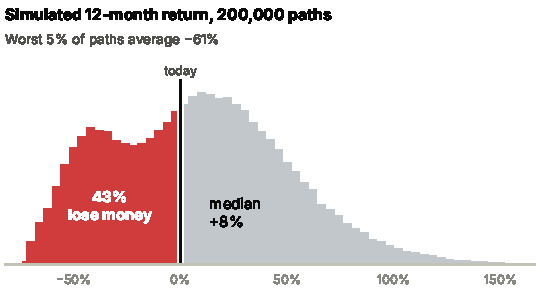
\includegraphics[width=0.72\columnwidth]{mc_returns.pdf}\par}
{\footnotesize Revenue sets both earnings and the multiple, which fattens the left tail. The mean is +8\%, below the 11\% (it's only a test of assumptions).}
 
Sizing: realized volatility is 84\% over 49 days (with the earnings gap) and 54\% over 20. Full Kelly is 0.20 to 0.25. We hold 1\% of the fund, about a twentieth of full Kelly. A 30\% fall costs the fund 0.3\%, and the worst-5\% outcome about 0.6\%.

\sect{6\quad Catalysts and signposts}
\begin{itemize}
\item Late Oct 2026: hyperscaler 2027 capex plans; Celestica reports Oct~26 (estimated).
\item Early Nov 2026 (Nov~2 estimated, not announced): FN FQ1. We want revenue of at least \$1{,}430M and an FQ2 guide midpoint of at least \$1{,}500M. Lumentum (laser supply) reports Nov~5.
\item Early 2027: Building~10 completion; FQ2 report (Feb) near 8\% q/q.
\item Rolling: street FY28 EPS moving toward \$24; FN named in a CPO chain.
\end{itemize}

\end{multicols}

\vspace{-4pt}
{\color{rule}\hrule height 0.4pt}
\vspace{2pt}
{\scriptsize\color{black!70}
Sources (checked Oct 6, 2026): [1] FN 8-K releases FQ1 to FQ4 FY26, SEC EDGAR. [2] FN FQ4 FY26 earnings call, Aug 17, 2026. [3] S\&P Global consensus via StockAnalysis.com (updated Sep 23; FY28 EPS single source). [4] FN daily prices, StockAnalysis.com. [5] FQ4 reaction coverage, TIKR. [6] FQ3 FY26 call summary. [7] optics.org, Mar 3, 2026. [8] Guidance in each prior 8-K. [9] StorageReview, Aug 15, 2026. [10] TrendForce via I/O Fund. [11] Forward P/E, StockAnalysis.com, Oct 5 close. [12] Deutsche Bank note via FinanceFeeds, Oct 1, 2026. Reverse DCF, scenarios, simulations: author's model (montecarlo.py, gbm.py). Fiscal year ends late June. Educational use in a student fund; not investment advice.\par}

% ================================================================= PAGE 2
\newpage
{\sffamily
\begin{tabularx}{\textwidth}{@{}X r@{}}
{\Large\bfseries\color{navy} Appendix: what the price path says about this trade} & {\small Long FN \textbar{} page 2}
\end{tabularx}}
\vspace{1pt}
{\color{rule}\hrule height 0.4pt}
\vspace{5pt}
 
{\small
100,000 daily price paths over 12 months (geometric Brownian motion), drift $\ln(515/453.84)=12.6\%$ as if our target is right, volatility 65\%. Realized volatility is 54\% over 20 trading days and 84\% over 49 (68\% without the Aug~18 gap). Options-implied volatility was not checked. The model has no revenue or margins, so it does not test the thesis. It sets what the price does regardless, and from that the entry price and the size.
 
\vspace{3pt}
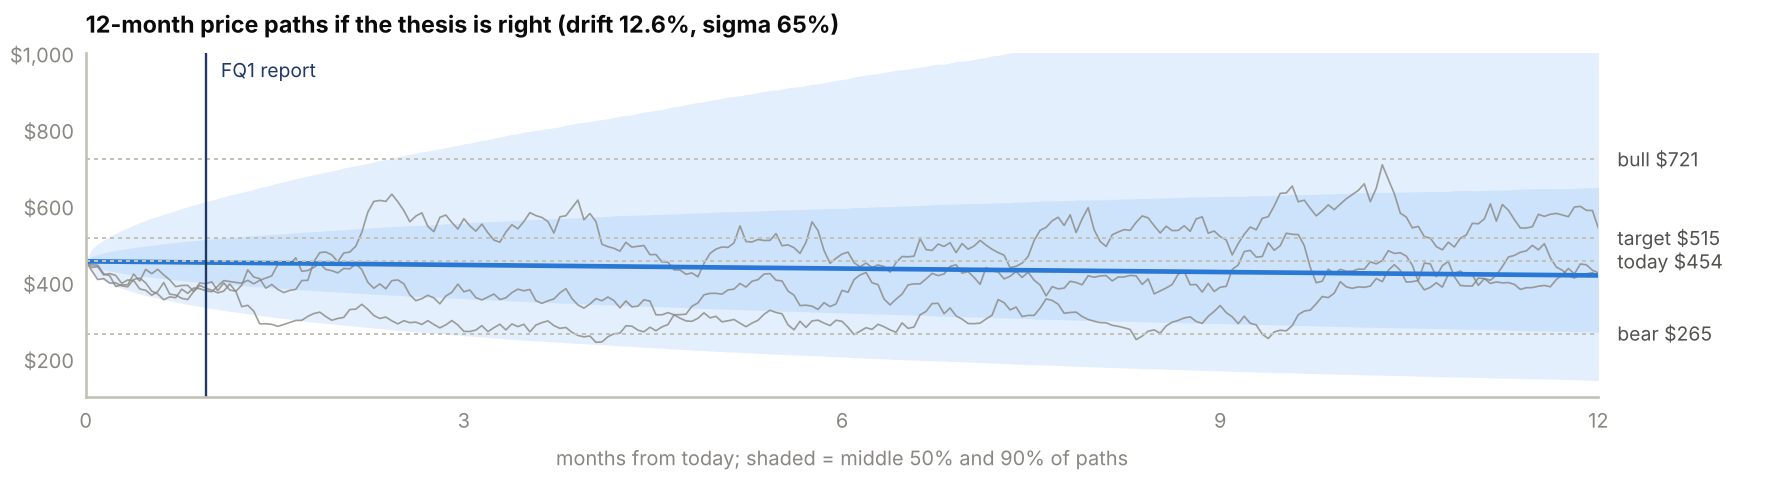
\includegraphics[width=\textwidth]{gbm_page2.png}
\vspace{1pt}
 
\begin{multicols}{2}
 
\sect{A\quad Even if we are right, the year is rough}
\begin{tabularx}{\columnwidth}{@{}X r@{}}
\toprule
Over 12 months & Share of paths\\
\midrule
Ends below today's \$454 & 55\%\\
Trades at \$515 at some point & 79\%\\
Ends the year above \$515 & 37\%\\
Trades at the \$265 bear value & 43\%\\
\bottomrule
\end{tabularx}
{\footnotesize Mean return +13.6\%, median $-$8.1\%: volatility costs $\sigma^2/2=21$ points of compound return. At 55\% and 75\% volatility the chance of a loss is 52\% and 58\%.}
 
\sect{B\quad The price before the report is noise}
One standard deviation over the 20 trading days to the estimated Nov~2 report is 18\% (\$378 to \$545), and the stock is at or above \$515 on report day in 24\% of paths. FN fell 19.4\% on Aug~18 when options priced 9.7\%. The thesis is tested by the FQ2 guide: street-consistent midpoint about \$1{,}420M, ours about \$1{,}490M. We exit below \$1{,}450M and treat \$1{,}500M or more as confirmation.
 
\columnbreak
 
\sect{C\quad The edge is thin at \$454 and wide below \$430}
\begin{tabularx}{\columnwidth}{@{}X rrrr@{}}
\toprule
Entry & To target & Bull/bear & Edge & Kelly\\
\midrule
\$417 & +23.5\% & 2.0$\times$ & +10.1 pts & 0.40\\
\$430 & +19.8\% & 1.8$\times$ & +7.0 pts & 0.33\\
\$454 (today) & +13.5\% & 1.4$\times$ & +1.6 pts & 0.20\\
\$464 & +11.1\% & 1.3$\times$ & $-$0.5 pts & 0.15\\
\bottomrule
\end{tabularx}
{\footnotesize Edge is $\ln(515/\mathrm{price})$ minus the 11\% holders require. Kelly is $(\mu-r)/\sigma^2$ with cash at 4\%.}
 
Above about \$460 the trade does not clear 11\% on our own numbers, so we do not add there. Below \$430 we add.
 
\sect{D\quad Size: 1\% of the fund}
Full Kelly is 0.20 here and 0.25 on page~1, and both rest on a drift we cannot measure. We hold a twentieth of it.
 
\begin{tabularx}{\columnwidth}{@{}X r@{}}
\toprule
Cost to the fund at a 1\% weight & Loss\\
\midrule
30\% fall from a high (96\% of paths) & 0.3\%\\
Median worst drawdown, 52\% & 0.5\%\\
Worst-5\% year, $-$75\% (page 1: $-$61\%) & 0.8\% (0.6\%)\\
\bottomrule
\end{tabularx}
 
\end{multicols}
}
 
\end{document}
 